\documentclass[a4paper, 11pt, english, fleqn]{article}
\usepackage[utf8]{inputenc}
\usepackage{babel}
%\usepackage{ngerman}
\usepackage{coordsys,logsys,color}
\usepackage{fancyhdr}
\usepackage{hyperref}
\usepackage{texdraw}				
\usepackage[T1]{fontenc}					
\usepackage{listings}
\usepackage{xcolor}
\usepackage{amsmath,amsfonts,amssymb}	
\usepackage[normalem]{ulem}	
\usepackage{listings}
\usepackage{graphicx}
\usepackage{enumitem}
\usepackage[paper=a4paper,left=35mm,right=35mm,top=35mm,bottom=30mm]{geometry}
\usepackage{graphicx,pifont}
\usepackage{wrapfig}

\let\oldding\ding
\renewcommand{\ding}[2][1]{\scalebox{#1}{\oldding{#2}}}

\hypersetup{colorlinks=true, breaklinks=true, linkcolor=darkblue, menucolor=black, urlcolor=darkblue, citecolor=darkblue}

\pagestyle{fancy}

\renewcommand{\familydefault}{cmss}

\definecolor{fgcgray}{rgb}{0.4, 0.4, 0.4}
\definecolor{darkblue}{rgb}{0,0, 0.4}
\newcommand{\titlefont}[1]{\textcolor{black}{\fontseries{bx}\fontshape{n}\fontsize{30}{0pt} \selectfont #1}}
\newcommand{\titlepagef}[1]{\textcolor{black}{\fontseries{bx}\fontshape{n}\fontsize{14}{0pt} \selectfont #1}}

\newcommand{\gloss}[1]{\textcolor{glossb}{\fontsize{11}{0pt}\selectfont #1}}

\newlist{aims}{enumerate}{1}
\setlist[aims,1]{
	label={Aim~\arabic*},
	leftmargin=*,
	align=left,
	%labelsep=1mm,
	font=\bfseries
}

\addtolength{\oddsidemargin}{-1.0cm}
\addtolength{\evensidemargin}{-1.0cm}
\addtolength{\headwidth}{2.0cm}
\addtolength{\textwidth}{2.0cm}

\setlength{\parindent}{0cm}

\renewcommand{\labelitemi}{$\circ$}
\renewcommand{\labelitemii}{$\diamond$}

\newcommand{\spaceline}[1][8pt]{\vskip #1}
\newcommand{\attrname}[1]{\textcolor{fgcgray}{\scriptsize #1}}

\newcommand{\comment}[1]{\spaceline[5pt] \textcolor{fgcgray}{\scriptsize #1} \spaceline[15pt]}

\makeatletter

\newcommand*{\project}[1]{\gdef\@project{#1}}


\def\@maketitle{
  %\begin{titlepage}
   
  \begin{center}
      \titlepagef{Software-Project 2017}
      \spaceline
  \end{center}
  
  \begin{center}
      \parbox{\textwidth}{
        \spaceline
        \centering{\titlefont{User Guide}}
        \par
        \spaceline
      }
  \end{center}
  
  \begin{center}
  	\titlepagef{Real-Time Mesh Utilities}
  	\spaceline[2em]
  \end{center}
  
  \begin{center}
  \begin{tabbing}
  Petros Simidyan \qquad \=
  Blerta Hamzallari \qquad \=
  Felix Griesau \qquad \=
  Marco Klamke \\
  Julius Lerm
  \>Lars Debor
  \>Simon Heinke  
  \>Sugandha Sachdeva
  \end{tabbing}
  \end{center}
 
  
  \spaceline[3em] {
    \begin{flushright}
    \begin{tabular}[t]{rl}
      \attrname{last change:} & \@date
    \end{tabular}
    \end{flushright}
    \par
  }
  \spaceline[5.5em]
  %\end{titlepage}
}

\begin{document}

\pagenumbering{gobble}
	
\lhead{\sc{User Guide: RTMU}}	
\title{User Guide: RTMU}
\vspace{3 in}
\maketitle


\includegraphics[width = \linewidth]{figures/mne-cpp.png}

\clearpage

\pagenumbering{arabic}

\tableofcontents

\clearpage

\lstset { %
	language=C++,
	backgroundcolor=\color{black!5}, % set backgroundcolor
	basicstyle=\footnotesize,% basic font setting
}

\section{Installation}

Since the project integrates into MNE-CPP and thus is directed at developers, there are no precompiled binaries or programs to install. The following tutorial explains all necessary steps to download and work with the results of this software project.

\begin{aims}
	\item[\hspace*{11mm} Qt Framework] Because MNE-CPP depends on the Qt framework, it must be installed. Therefore, you must download and install it.
\end{aims}

\begin{aims}
	\item[\hspace*{11mm} MNE-CPP Source Code] We recommend using Git to get the MNE-CPP source code, as you can simply clone / fork one of MNE-CPP's repositories.
\end{aims}

\begin{aims}
	\item[\hspace*{11mm} Compiling the Source Code] Since Qt creator is automatically installed when you install the Qt framework, it is easiest to use its build-in compiler. You must first run the \textit{mne-cpp.pro} file, then run \textit{qmake} and finally start a build of the project. After this, all binaries can be found inside the \textit{bin} folder.
\end{aims}

For more details, see \url{http://wiki.mne-cpp.org/index.php/Portal:Getting_Started}.

\clearpage

\section{Detailed Example}

This section should illustrate the use of the classes \textit{GeometryInfo} and \textit{Interpolation} by providing a detailed example.

\subsection{GeometryInfo}

This class provides three features: sensor-to-mesh mapping, surface constrained distance calculation and bad channel filtering.

\subsubsection{Sensor Projecting}

The method \textit{GeometryInfo::projectSensors} allows sensor-to-mesh mapping. This is needed because sensor positions may be somewhat above the vertices of the used mesh:\\
\begin{figure}[h]
	\begin{center}
		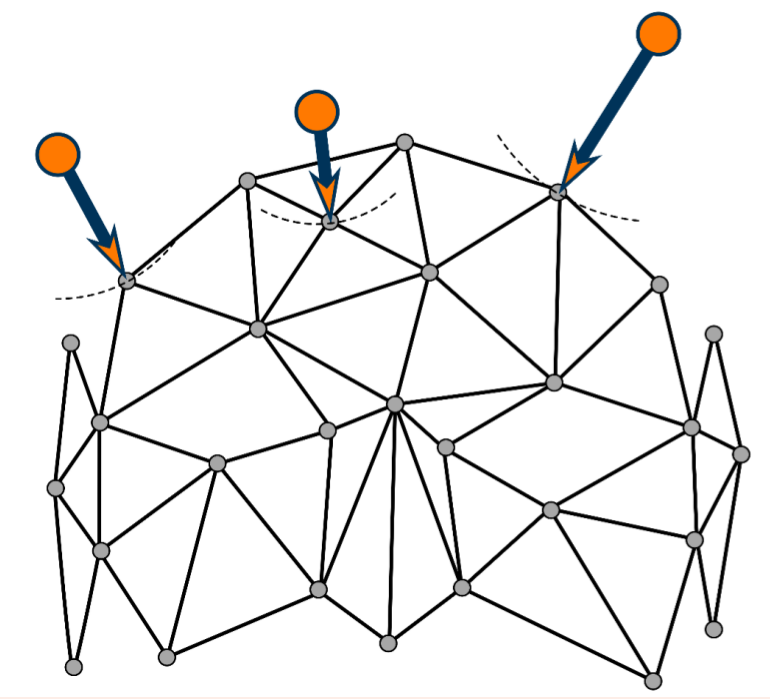
\includegraphics[width=10cm]{figures/sensorToMeshMapping.png}
		\caption{Sensor must be assigned to the best-matching vertex}
	\end{center}
\end{figure}
\\
The method receives two arguments: one MNEBemSurface and a QVector of Vector3f objects (Eigen representation of 3D coordinates). Said vector must contain the absolute positions of the sensors in 3D space.\\
Thus, a MNEBemSurface must be obtained first: 
\begin{lstlisting}
// extract MNEBemSurface from file
QFile t_filesensorSurfaceVV(QDir::currentPath()
		+ "/mne-cpp-test-data/subjects/sample/bem/sample-5120-bem.fif");
MNEBem t_sensorSurfaceVV(t_filesensorSurfaceVV);
MNEBemSurface surface = t_sensorSurfaceVV[0];
\end{lstlisting}

After that the sensor positions must be extracted:

\begin{lstlisting}
// extract FiffEvoked object from file
QFile t_fileEvoked(QDir::currentPath()
			+ "/mne-cpp-test-data/MEG/sample/sample_audvis-ave.fif");
fiff_int_t setno = 0;
QPair<QVariant, QVariant> baseline(QVariant(), 0);
FiffEvoked evoked = FiffEvoked(t_fileEvoked, setno, baseline);

// for MEG sensors (use magnetometers only)
QVector<Vector3f> megSensors;

for( const FiffChInfo &info : evoked.info.chs) {
	if(info.kind == FIFFV_MEG_CH && info.unit == FIFF_UNIT_T) {
		megSensors.push_back(info.chpos.r0);
	}
}


// for EEG sensors
QVector<Vector3f> eegSensors;
    
for( const FiffChInfo &info : evoked.info.chs) {
	if(info.kind == FIFFV_EEG_CH && info.unit == FIFF_UNIT_V) {
		eegSensors.push_back(info.chpos.r0);
	}
}
\end{lstlisting}

\begin{center}
\textit{Note: EEG sensors may need co-registration.}
\end{center}

The method \textit{GeometryInfo::projectSensors} returns a pointer to a vector of indices that point to the best matching vertices of the passed mesh:
\begin{lstlisting}
 QSharedPointer<QVector<qint32>> pVecMappedSubset;
 pVecMappedSubset = GeometryInfo::projectSensors(surface, megSensors);
\end{lstlisting}

A very simplified example further illustrates this:

\begin{figure}[h]
	\begin{center}
		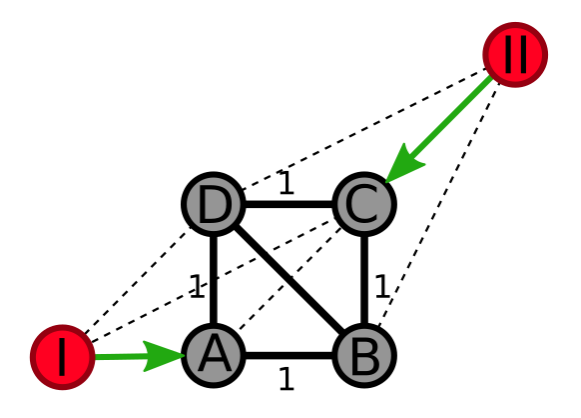
\includegraphics[width=6cm]{figures/sensorMappingSimpleBefore.png}
		\caption{Sensors are red, A-D are vertex IDs / indices}
	\end{center}
\end{figure}

%this is just to fix umbrueche
\clearpage

The algorithm would map the sensors as follows:

\begin{figure}[h]
	\begin{center}
		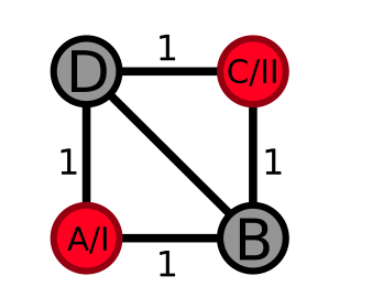
\includegraphics[width=5cm]{figures/sensorMappingSimpleAfter.png}
		\caption{Mapped sensors}
	\end{center}
\end{figure}

The output vector thus would be:
\[
\begin{pmatrix} A & C \end{pmatrix}
\]

\subsubsection{Surface Constrained Distance Calculation}

In order to interpolate signals, distances between vertices are of significant interest. Because using euclidian distances for further calculations is very imprecise, we provided a method for calculating surface constrained distances.

\begin{figure}[h]
	\centering
	\begin{minipage}[b]{0.46\textwidth}
		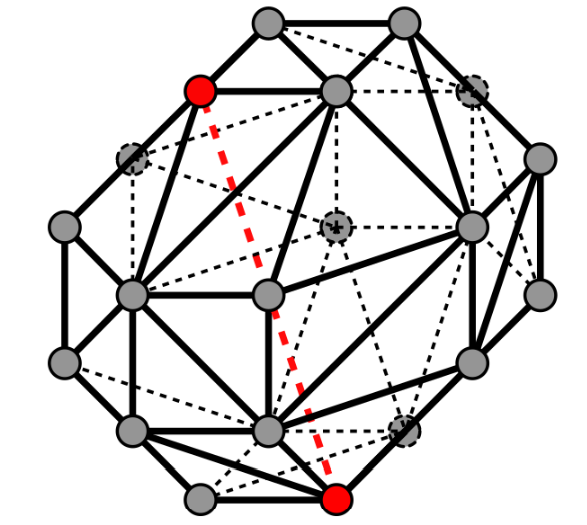
\includegraphics[width=\textwidth]{figures/scdcEuclid.png}
		\caption{Euclidian distance}
	\end{minipage}
	\hfill
	\begin{minipage}[b]{0.46\textwidth}
		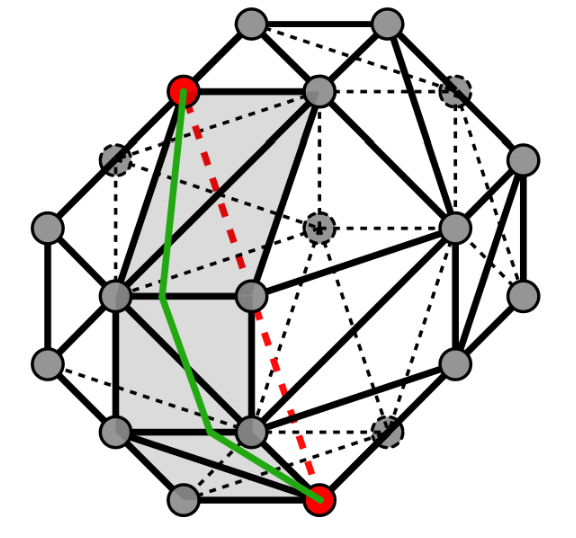
\includegraphics[width=\textwidth]{figures/scdcPrecise.png}
		\caption{Precise SCD}
	\end{minipage}
\end{figure}

%this is just to fix the umbrueche
\clearpage

Since precise calculation of surface constrained distances takes far too much computation time, we decided to approximatively calculate distances by using the edges of the mesh:

\begin{figure}[h]
	\begin{center}
		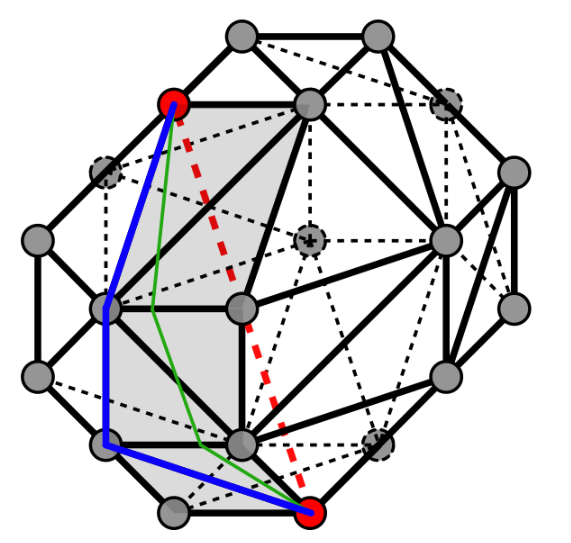
\includegraphics[width=8cm]{figures/scdcEdges.png}
		\caption{Approximating SCDs via shortest path on edges}
	\end{center}
\end{figure}

To further reduce computation time, we introduced a distance threshold: Vertices with a higher distance than said threshold are assumed to be infinitely far away from one another.

\begin{figure}[h]
	\begin{center}
		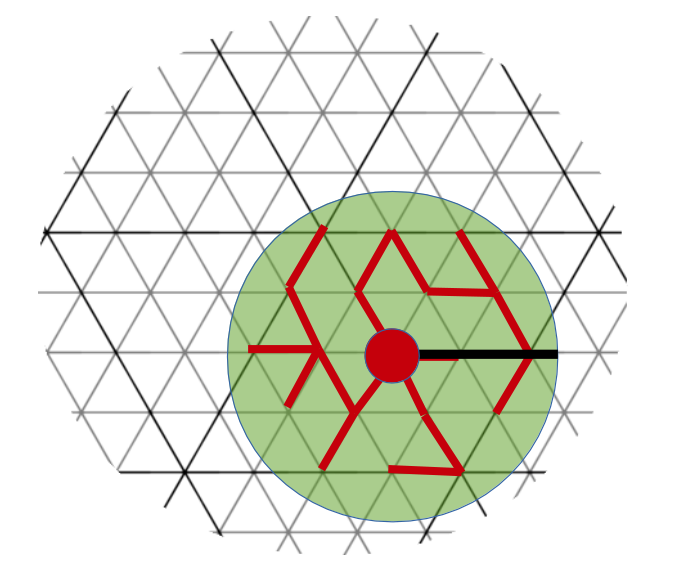
\includegraphics[width=8cm]{figures/cancelDist.png}
		\caption{Distances are only calculated inside the radius of the distance threshold(black)}
	\end{center}
\end{figure}

The method \textit{GeometryInfo::scdc} receives three arguments: a MNEBemSurface that holds the mesh, a vector of indices (see Sensor Projecting for more details) and the distance treshold. The second argument represents the indices that distances should be calculated to (in most cases this is the result of the sensor mapping). An empty vector can be passed to indicate that all distances (all pairs) should be calculated. Duly note that this can consume a significantly large amount of memory. The method outputs a pointer to a matrix that holds all calculated distance values.\\
\\
Since the third argument, i.e. the distance threshold is defaulted with infinity, it can be left out in case the full distance table is wanted. Duly note that this may take a considerable amount of time.

\begin{figure}[h]
	\centering
	\begin{minipage}[b]{0.56\textwidth}
		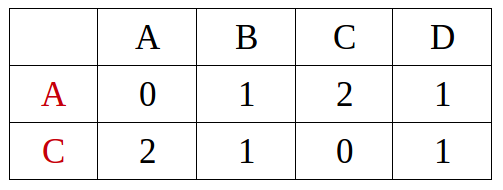
\includegraphics[width=\textwidth]{figures/distanceTableWithoutCanceldist.png}
		\caption{All distances are calculated}
	\end{minipage}
	\hfill
	\begin{minipage}[b]{0.36\textwidth}
		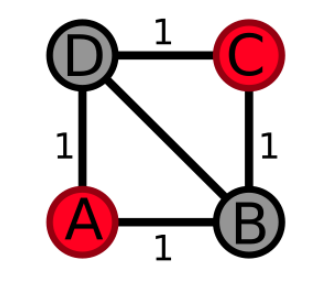
\includegraphics[width=\textwidth]{figures/meshSCDC.png}
		\caption{A and C are of interest here}
	\end{minipage}
\end{figure}

\begin{figure}[h]
	\centering
	\begin{minipage}[b]{0.56\textwidth}
		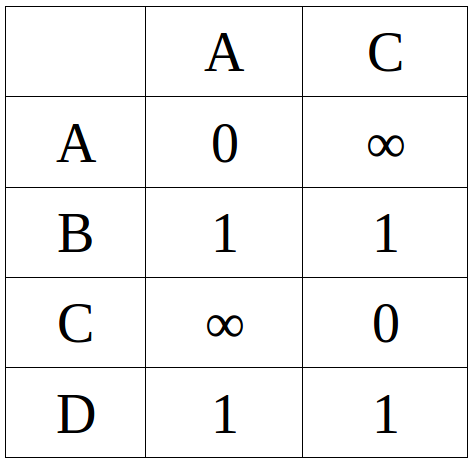
\includegraphics[width=\textwidth]{figures/distanceTableWithCanceldist.png}
		\caption{Result of \textit{scdc} with a distance threshold of 1.5 cm}
	\end{minipage}
	\hfill
	\begin{minipage}[b]{0.36\textwidth}
		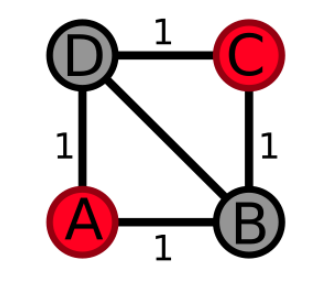
\includegraphics[width=\textwidth]{figures/meshSCDC.png}
		\caption{A and C are of interest here}
	\end{minipage}
\end{figure}

\begin{lstlisting}
// scdc with distance threshold of 3cm
QSharedPointer<MatrixXd> distanceTable;
distanceTable = GeometryInfo::scdc(surface, pVecMappedSubset, 0.03);
\end{lstlisting}

\subsubsection{Bad Channel Filtering}

Since some sensors produce corrupted or distorted signals, they are marked as bad. These bad channels must be excluded from further computations, because they would distort the interpolation otherwise. The method \textit{GeometryInfo::filterBadChannels} achieves this by setting the distance values for bad sensors to infinity. This way, the bad sensors are assumed to have an infinite distance to every other vertex of the mesh and thus to have no influence on them when interpolating.\\
The method receives three arguments: the distance table, a FiffInfo object that holds the bad channel information and the type of the used sensors.

\begin{lstlisting}
// filter for bad MEG channels:
QVector<qint32> erasedColums;
erasedColumns = GeometryInfo::filterBadChannels(distanceTable,
						evoked.info,
						FIFFV_MEG_CH);
\end{lstlisting}

A simplified result of such a filtering could look like this (assume that A, B, C are sensors and B is bad).

%@todo include grapic

\subsection{Interpolation}

This class provides two features: creation of weight matrices / interpolation matrices and interpolation of sensor signals.

\subsubsection{Weight Matrix Creation}

The method \text{GeometryInfo::createInterpolationMat} receives six arguments: a vector of vertex IDs, a distance table, a pointer to a function, a distance threshold, a FiffInfo object and a sensor type. The first argument must be the result of Sensor Projecting in order to get correct results. The pointer to the function determines what function is used for evaluating influence of sensor vertices. The distance threshold has the same function as in the SCDC method: coefficients for vertices with higher distances than this are set to zero. Since bad channels must be considered during the calculation of the weight matrix, a FiffInfo object must be passed. Lastly the used sensor type must be passed. 

\begin{lstlisting}
// weight matrix creation
QSharedPointer<SparseMatrix<double> > weights;
weights = Interpolation::createInterpolationMat(pVecMappedSubset,
						distanceTable,
						Interpolation::linear,
						0.20,
						evoked.info,
						FIFFV_MEG_CH);
\end{lstlisting}

The method outputs a pointer to a matrix that holds the interpolation coefficients for all vertices.\\
Assume that we have 49 vertice but only 2 sensors. The following figure illustrates how each vertex is influenced by the two sensors.

\begin{figure}[h]
	\begin{center}
		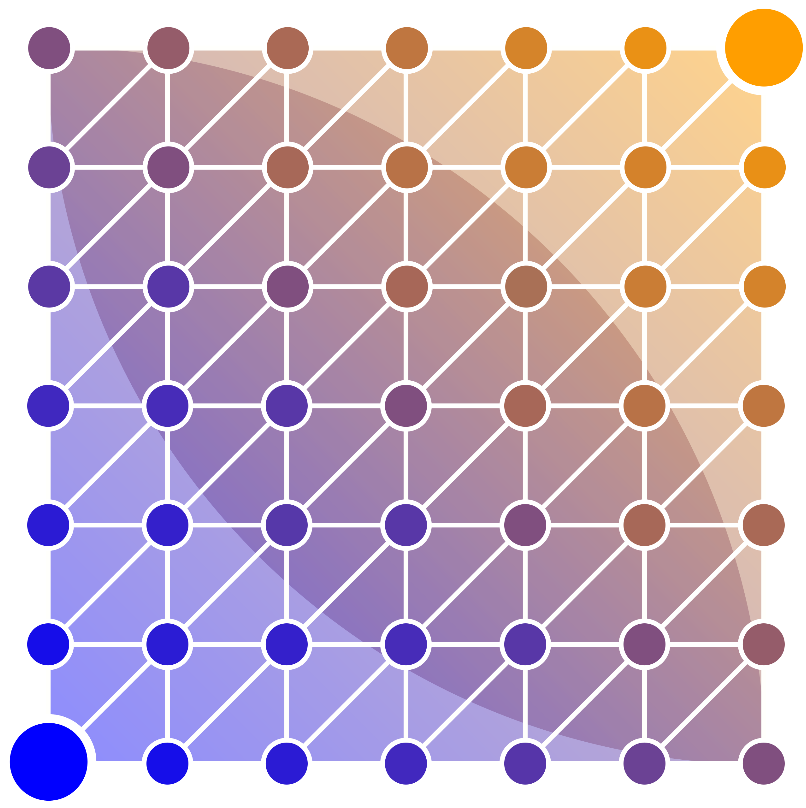
\includegraphics[width=8.5cm]{figures/coefficients.png}
		\caption{Influence of two sensors}
	\end{center}
\end{figure}

\subsubsection{Signal Interpolation}

The method \textit{Interpolation::interpolateSignal} receives two arguments: a weight matrix and a vector that represents the respective sensor signal. It outputs a vector with interpolated values for each vertex of the used mesh.

\begin{lstlisting}
// random data set
VectorXd testSignal = VectorXd::Random(pVecMappedSubset->size());

// interpolate with random data set
QSharedPointer<VectorXf> interpolatedSignal;
interpolatedSignal = Interpolation::interpolateSignal(weights, testSignal);
\end{lstlisting}

Assume that we have the following weight matrix
\begin{figure}[h]
	\begin{center}
		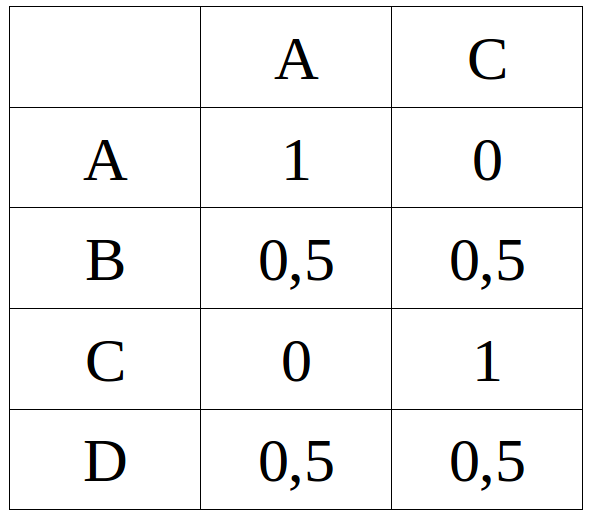
\includegraphics[width=5cm]{figures/weights.png}
		\caption{Influence of two sensors A and C}
	\end{center}
\end{figure}

and the following sensor signal:
\begin{figure}[ht]
	\centering
	$\begin{pmatrix}
	100 \\ 0
	\end{pmatrix}$
\end{figure}


The output then would be this vector:
\begin{figure}[ht]
	\centering
	$
	\begin{pmatrix} 100 \\ 50 \\ 0 \\ 50 \end{pmatrix}
	$
\end{figure}

\clearpage


\clearpage
\section{Navigation in Disp3D}

This section describes how to navigate through the 3D control widget of the Disp3D example.

\begin{aims}
	\item[\hspace*{10mm} Where to Navigate] The two new items that use the new features can be found under\\ \textit{sample/Right visual/MEG Data} \ding[1.4]{182} and \textit{sample/Right visual/EEG Data}. \ding[1.4]{183} \\ 
	MEG data utilizes the Sensor Surface under \textit{Sensors/VectorView/Sensor Surface} \ding[1.4]{182}, while EEG data uses the Head surface under \textit{sample/BEM/Head}. \ding[1.4]{183} 
\end{aims}
	
	
\begin{aims}
	\item[\hspace*{10mm} Turning Data Streams On/Off] Click the checkbox "Stream data on/off" to toggle data streaming. All necessary calculations are executed and the interpolation begins. \ding[1.4]{184}
\end{aims}

\begin{aims}
	\item[\hspace*{10mm} Choosing a Color Map] Click on the second row of text and then choose an entry of the droplist to switch color maps. \ding[1.4]{185}
\end{aims}

\begin{aims}
	\item[\hspace*{10mm} Configuring Normalization Thresholds] Click on the third row of text and then click left inside the arising graph for the lower threshold and right for the upper threshold. 
	Unwanted activation can be hidden this way. \ding[1.4]{186}
\end{aims}

\begin{aims}
	\item[\hspace*{10mm} Editing sample delays] Use the spinbox in the fourth row to decrease / increase the delay between visual outputs. \ding[1.4]{187}
\end{aims}

\begin{aims}
	\item[\hspace*{10mm} Toggling Data Looping] Click the checkbox in the fifth row to toggle looping of the last received block of sensor data. \ding[1.4]{188}
\end{aims}

\begin{aims}
	\item[\hspace*{10mm} Sample Averaging] Use the spinbox in the sixth row to decrease / increase the number of samples that should be averaged to one signal. \ding[1.4]{189}
\end{aims}

\begin{aims}
	\item[\hspace*{10mm} Distance Threshold] Use the spinbox in the seventh row to decrease / increase the distance threshold that is used when running the SCDC and the creation of the interpolation matrix. By doing this less / more vertices around the sensor locations are considered during  the interpolation. \ding[1.4]{190}
\end{aims}

\begin{aims}
	\item[\hspace*{10mm} Interpolation Function] Use the droplist in the last row to choose a function to use during the creation of the interpolation matrix. \ding[1.4]{191}
\end{aims}



  
\end{document}
